\noindent
En el mundo actual, en el que la informática gira en torno al concepto de red, el trabajo de los administradores de sistemas es muy complejo. Su misión consiste en mantener en funcionamiento recursos tales como encaminadores (routers), concentradores (hubs), switches, servidores, así como cada dispositivo crítico que conforma la red. 
Hay gran cantidad de motivos por los cuales un administrador necesita monitorizar entre otros : la utilización del ancho de banda, el estado de funcionamiento de los enlaces, la detección de cuellos de botella, detectar y solventar problemas con el cableado, administrar la información de encaminamiento entre máquinas, etc. La monitorización de la red es también un buen punto desde el que comenzar el estudio de los problemas de seguridad.

\noindent
En muchos casos, la red de una organización está enlazada mediante costosos enlaces a redes de área extensa (WAN) o con la Internet, y cuyos costes dependen del volumen de tráfico. Es muy importante mantener un registro estadístico del tráfico que circula por estos enlaces. Ésta situación es bastante común en Europa, donde los enlaces X.25 son todavía de uso corriente. La tarificación de este tipo de líneas se realiza en función del número de paquetes enviados y recibidos. La respuesta a lo anteriormente planteado es el protocolo SNPM. \cite{intro_snmp}

% ==========================================================================================================================
\section{SNMP}
% ==========================================================================================================================

\noindent
El protocolo llamado Simple Network Management Protocol (SNMP), es un protocolo diseñado en los años 80, su principal objetivo fue el integrar la gestión de diferentes tipos de redes mediante un diseño sencillo y que produjera poca sobrecarga en la red.
SNMP opera en el nivel de aplicación, utilizando el protocolo de transporte TCP/IP, por lo que ignora los aspectos específicos del hardware sobre el que funciona. La gestión se lleva a cabo al nivel de IP, por lo que se pueden controlar dispositivos que estén conectados en cualquier red accesible desde la Internet, y no únicamente aquellos localizados en la propia red local. Evidentemente, si alguno de los dispositivos de encaminamiento con el dispositivo remoto a controlar no funciona correctamente, no será posible su monitorización ni reconfiguración.

\noindent
\newline
El protocolo SNMP está compuesto por dos elementos: el agente (agent), y el gestor (manager). Es una arquitectura cliente-servidor, en la cual el agente desempeña el papel de servidor y el gestor hace el de cliente
\noindent
El agente es un programa que ha de ejecutase en cada nodo de red que se desea gestionar o monitorizar. Ofrece un interfaz de todos los elementos que se pueden configurar. Estos elementos se almacenan en unas estructuras de datos llamadas "Management Information Base" (MIB), se explicarán más adelante. Representa la parte del servidor, en la medida que tiene la información que se desea gestionar y espera comandos por parte del cliente.
\noindent
El gestor es el software que se ejecuta en la estación encargada de monitorizar la red, y su tarea consiste en consultar los diferentes agentes que se encuentran en los nodos de la red los datos que estos han ido obteniendo.

\noindent
\newline
En esencia, el SNMP es un protocolo muy sencillo puesto que todas las operaciones se realizan bajo el paradigma de carga-y-almacenamiento (load-and-store), lo que permite un juego de comandos reducido. Un gestor puede realizar sólo dos tipos diferentes de operaciones sobre un agente: leer o escribir un valor de una variable en el MIB del agente. Estas dos operaciones se conocen como petición-de-lectura (get-request) y petición-de-escritura (set-request). Hay un comando para responder a una petición-de-lectura llamado respuesta-de-lectura (get-response), que es utilizado únicamente por el agente.
\noindent
La posibilidad de ampliación del protocolo está directamente relacionado con la capacidad del MIB de almacenar nuevos elementos. Si un fabricante quiere añadir un nuevo comando a un dispositivo, como puede ser un encaminador, tan sólo tiene que añadir las variables correspondientes a su base de datos (MIB).
\noindent
Casi todos los fabricantes implementan versiones agente de SNMP en sus dispositivos: encaminadores, hubs, sistemas operativos, etc. Linux no es una excepción, existen varios agentes SNMP disponibles públicamente en la Internet. \cite{intro_snmp}

\noindent	
\newline
La versión original, ahora conocido como SNMPv1, es ampliamente difundida. SNMPv2 añade funcionalidad a la versión original, pero no se ocupa de sus limitaciones de seguridad; esta norma relativamente reciente no ha alcanzado mucha aceptación. La versión SNMPv3 que conserva las mejoras funcionales de SNMPv2 y añade potentes funciones de privacidad y autenticación.
El protocolo simple de administración de red (SNMP), publicado en 1988, fue diseñado para proporcionar una implementación sencilla, así como facilitar el trabajo de gestión de redes de múltiples proveedores (enrutadores, servidores, estaciones de trabajo y otros recursos de la red). 

\noindent
\newline
La especificación de SNMP tiene como objetivo:
\begin{itemize}
	\item Definir un protocolo para el intercambio de información entre uno o más sistemas de gestión y un número de agentes,
	\item Proporcionar un marco para dar formato y almacenamiento de información de gestión y
	\item Define una serie de variables de información de gestión de propósito general, u objetos.
\end{itemize}

\noindent
La versión original de SNMP (ahora conocido como SNMPv1) se convirtió rápidamente en el esquema de gestión de la red más utilizado. Sin embargo, como el uso del protocolo se generalizó, se hicieron evidentes sus deficiencias. Estas incluyen la falta de comunicación-manager-manager, la incapacidad para hacer la transferencia de datos a granel, y la falta de seguridad. 

\noindent
\newline
SNMPv2 no ha recibido la aceptación que sus diseñadores anticiparon. Mientras que las mejoras funcionales han sido bienvenidas, los desarrolladores encontraron las modificaciones de seguridad para SNMPv2 demasiado complejas. En consecuencia, el grupo de trabajo SNMPv2 se reactivó para proporcionar una mejora de los documentos SNMPv2.
El resultado de este esfuerzo ha sido un éxito menor y un gran fracaso. El éxito de menor importancia es la mejora de los aspectos funcionales de SNMPv2. El gran fracaso radica en el área de la seguridad. El grupo de trabajo fue incapaz de resolver el problema, y surgieron dos enfoques diferentes. Con esta mejora, la parte funcional de SNMPv2 progresó de una propuesta a un estándar de Internet a partir de 1996. Luego, en 1997, empezó a trabajar en SNMPv3, lo que hace cambios funcionales menores e incorpora un nuevo enfoque de seguridad.

\begin{figure}[htbp!]
	\centering
		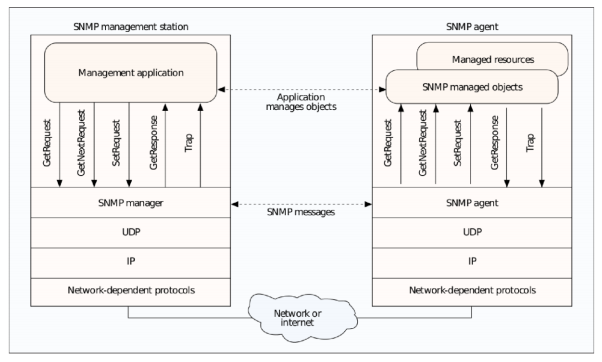
\includegraphics[width=0.8\textwidth]{images/introduccion/snmp}
	\caption{Agente y gestor SNMP.}
\end{figure}

% ==========================================================================================================================
\subsection{¿Qué es la MIB}
% ==========================================================================================================================

\noindent
SNMP define un estándar separado para los datos gestionados por el protocolo. Este estándar define los datos mantenidos por un dispositivo de red, así como las operaciones que están permitidas. Los datos están estructurados en forma de árbol; en el que sólo hay un camino desde la raíz hasta cada variable. Esta estructura en árbol se llama Management Information Base (MIB) y se puede encontrar información sobre ella en varios RFC's.
\noindent
La versión actual de TCP/IP MIB es la 2 (MIB-II) y se encuentra definida en el RFC-1213. En ella se divide la información que un dispositivo debe mantener en ocho categorías (ver Tabla 1). Cualquier variable ha de estar en una de estas categorías.

\begin{table}[htbp]
	\begin{center}
		\begin{tabular}{|l|l|}
		\hline
		Objeto. 			& Descripción. \\ \hline \hline
		System 				& Información del host del sistema de encaminamiento. 	\\ \hline
		Interfaces 			& Información de los interfaces de red. 				\\ \hline
		Address Translation & Información de traducción de direcciones. 			\\ \hline
		IP 					& Información sobre el protocolo IP. 					\\ \hline
		ICMP 				& Información sobre el protocolo ICMP. 					\\ \hline
		TCP 				& Información sobre el protocolo TCP. 					\\ \hline
		UDP 				& Información sobre el protocolo UDP. 					\\ \hline
		UGP 				& Información sobre el protocolo (Exterior Gateway). 	\\ \hline
		\end{tabular}
	\caption{Objetos de la MIB.}
	\label{tabla:objetos_mib}
	\end{center}
\end{table}

\noindent 
La definición de un elemento concreto MIB implica la especificación del tipo de dato que puede contener. Normalmente, los elementos de un MIB son enteros, pero también pueden almacenar cadenas de caracteres o estructuras más complejas como tablas. A los elementos de un MIB se les llama "objetos". Los objetos son los nodos hoja del árbol MIB, si bien, un objeto puede tener más de una instancia, como por ejemplo un objeto tabla. Para referirse al valor contenido en un objeto, se ha de añadir el número de la instancia. Cuando sólo exista una instancia del objeto, está es la instancia cero.
\noindent
Por ejemplo, el objeto ifNumber de la categoría "interfaces" es un entero que representa el número de interfaces presentes en el dispositivo; mientras el objeto ipRoutingTable de la categoría "ip" contiene la tabla de encaminamiento del dispositivo.
\noindent
Hay que acordarse de utilizar el número de la instancia para leer el valor de un objeto. En este caso, el número de interfaces presentes en un encaminador puede ser observado mediante la instancia ifNumber.0.
\noindent
En el caso de ser un objeto tabla, se ha de utilizar el índice a la tabla como último número para especificar la instancia (fila de la tabla).

\noindent
\newline
Existe otro estándar que define e identifica las variables MIB, llamado "Structure of Management Information" (SMI). SMI especifica las variables MIB, éstas se declaran empleando un lenguaje formal ISO llamado ASN.1, que hace que tanto la forma como los contenidos de estas variables sean no ambiguos.
\noindent
El espacio de nombres ISO (árbol) está situado dentro de un espacio de nombres junto con otros árboles de otros estándares de otras organizaciones. Dentro del espacio de nombres ISO hay una rama específica para la información MIB. Dentro de esta rama MIB, los objetos están a su vez jerarquizados en subárboles para los distintos protocolos y aplicaciones, de forma que esta información puede representarse unívocamente.
\noindent
La siguiente figura muestra el espacio de nombres del MIB del TCP/IP, éste está situado justo bajo el espacio del IAB "mgmt". La jerarquía también específica el número para cada nivel.

\begin{figure}[htbp!]
	\centering
		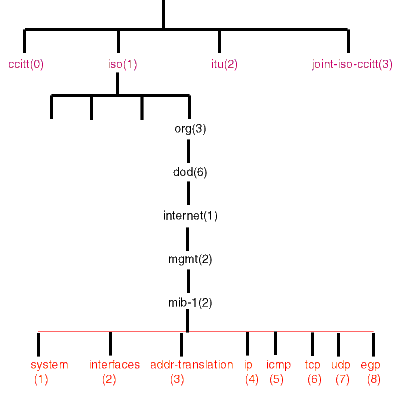
\includegraphics[width=0.8\textwidth]{images/introduccion/jerarquia}
	\caption{Jerarquía del árbol.}
\end{figure}

\noindent
Es importante constatar que la mayor parte del software necesita el punto raíz (.) para localizar el objeto en el MIB. Si no se incluye el punto raíz, se asume que el path es relativo desde .iso.org.dod.internet.mgmt.mib-2.
\noindent
De esta forma, el objeto ifNumber de la categoría "interfaces" se puede llamar: \textbf{.iso.org.dod.internet.mgmt.mib-2.interfaces.ifnumber} o el equivalente numérico: \textbf{.1.3.6.1.2.1.2.1}. Y la instancia es: \textbf{.iso.org.dod.internet.mgmt.mib-2.interfaces.ifnumber.0}
o el equivalente numérico: \textbf{.1.3.6.1.2.1.2.1.0}.
\noindent
Adicionales MIB se pueden añadir a este árbol conforme los vendedores definen nuevos objetos y publican los correspondientes RFC.